\documentclass[tikz, border=4pt]{standalone}
\usepackage{tikz}
\usetikzlibrary{arrows.meta, decorations.pathreplacing}
\begin{document}
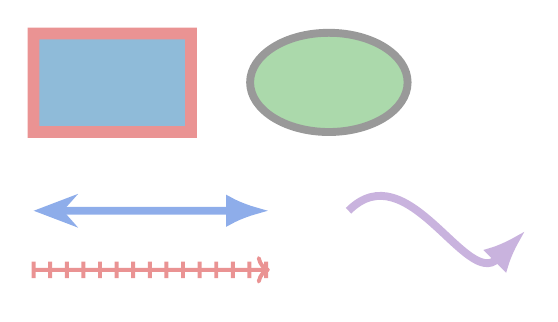
\begin{tikzpicture}[x=1cm, y=1cm]
  \definecolor{tdc1}{HTML}{D62728}
  \definecolor{tdc2}{HTML}{1F77B4}
  \definecolor{tdc3}{HTML}{2CA02C}
  \definecolor{tdc4}{HTML}{1E5BD6}
  \definecolor{tdc5}{HTML}{9467BD}

  \begin{scope}[transparency group, opacity=0.5]
    \draw[draw=tdc1, line width=4.27pt, fill=tdc2] (0,-1.25) rectangle (2,0);
  \end{scope}
  \begin{scope}[transparency group, opacity=0.4]
    \draw[line width=2.85pt, fill=tdc3] (3.75,-0.62) ellipse (1 and 0.63);
  \end{scope}
  \begin{scope}[transparency group, opacity=0.5]
    \draw[draw=tdc4, line width=2.85pt, {Stealth}-{Latex}] (0,-2.25) -- (3,-2.25);
  \end{scope}
  \begin{scope}[transparency group, opacity=0.5]
    \draw[draw=tdc1, line width=1.42pt, -{To}, postaction={draw, -, solid, decorate, decoration={ticks, segment length=6pt, amplitude=3pt}}] (0,-3) -- (3,-3);
  \end{scope}
  \begin{scope}[transparency group, opacity=0.5]
    \draw[draw=tdc5, line width=2.85pt, -{Latex}] (4,-2.25) .. controls (4.75,-1.5) and (5.5,-3.25) .. (6.25,-2.5);
  \end{scope}
\end{tikzpicture}
\end{document}
